\documentclass{beamer}
\usepackage[utf8]{inputenc}

\usetheme{Madrid}
\usecolortheme{default}
\usepackage{amsmath,amssymb,amsfonts,amsthm}
\usepackage{txfonts}
\usepackage{tkz-euclide}
\usepackage{listings}
\usepackage{adjustbox}
\usepackage{array}
\usepackage{tabularx}
\usepackage{gvv}
\usepackage{lmodern}
\usepackage{circuitikz}
\usepackage{tikz}
\usepackage{graphicx}

\setbeamertemplate{page number in head/foot}[totalframenumber]

\usepackage{tcolorbox}
\tcbuselibrary{minted,breakable,xparse,skins}



\definecolor{bg}{gray}{0.95}
\DeclareTCBListing{mintedbox}{O{}m!O{}}{%
  breakable=true,
  listing engine=minted,
  listing only,
  minted language=#2,
  minted style=default,
  minted options={%
    linenos,
    gobble=0,
    breaklines=true,
    breakafter=,,
    fontsize=\small,
    numbersep=8pt,
    #1},
  boxsep=0pt,
  left skip=0pt,
  right skip=0pt,
  left=25pt,
  right=0pt,
  top=3pt,
  bottom=3pt,
  arc=5pt,
  leftrule=0pt,
  rightrule=0pt,
  bottomrule=2pt,
  toprule=2pt,
  colback=bg,
  colframe=orange!70,
  enhanced,
  overlay={%
    \begin{tcbclipinterior}
    \fill[orange!20!white] (frame.south west) rectangle ([xshift=20pt]frame.north west);
    \end{tcbclipinterior}},
  #3,
}
\lstset{
    language=C,
    basicstyle=\ttfamily\small,
    keywordstyle=\color{blue},
    stringstyle=\color{orange},
    commentstyle=\color{green!60!black},
    numbers=left,
    numberstyle=\tiny\color{gray},
    breaklines=true,
    showstringspaces=false,
}
%------------------------------------------------------------

\title
{2.9.22}
\date{September 8,2025}
\author 
{AI25BTECH11006 - Nikhila}



\begin{document}


\frame{\titlepage}
\begin{frame}{Question}
 Let $\overrightarrow{a}$,
$\overrightarrow{b}$, and $\overrightarrow{c}$ be three vectors such that $|\overrightarrow{a}|$ = 1, $|\overrightarrow{b}|$ = 2, and $|\overrightarrow{c}|$ = 3. If the
projection of $\overrightarrow{b}$ along $\overrightarrow{a}$ is equal to the projection of $\overrightarrow{c}$ along $\overrightarrow{a}$, and $\overrightarrow{b}$ and $\overrightarrow{c}$ are perpendicular to each other, then find $|3\overrightarrow{a} - 2\overrightarrow{b} + 2\overrightarrow{c}|$.
\end{frame}


\begin{frame}[fragile]
    \frametitle{Theoretical Solution using Gram Matrix}
We are given:
\[
\norm{\vec{a}} = 1, \quad \norm{\vec{b}} = 2, \quad \norm{\vec{c}} = 3
\]
with conditions
\[
\vec{a}^T\vec{b} = \vec{a}^T\vec{c}, \quad \vec{b}^T\vec{c} = 0
\]

\textbf{Step 1: Construct Gram matrix.}

\[
G =
\begin{bmatrix}
\vec{a}^T\vec{a} & \vec{a}^T\vec{b} & \vec{a}^T\vec{c} \\
\vec{b}^T\vec{a} & \vec{b}^T\vec{b} & \vec{b}^T\vec{c} \\
\vec{c}^T\vec{a} & \vec{c}^T\vec{b} & \vec{c}^T\vec{c}
\end{bmatrix}
=
\begin{bmatrix}
1 & x & x \\
x & 4 & 0 \\
x & 0 & 9
\end{bmatrix}
\]
where $x = \vec{a}^T\vec{b} = \vec{a}^T\vec{c}$.
\end{frame}


\begin{frame}[fragile]
\frametitle{Theoretical Solution using Gram Matrix}
\textbf{Step 2: Define vector combination.}

\[
\vec{v} = 3\vec{a} - 2\vec{b} + 2\vec{c}, \quad
\vec{u} =
\begin{bmatrix}
3 \\ -2 \\ 2
\end{bmatrix}
\]

\textbf{Step 3: Use Gram matrix to compute norm.}

\[
\norm{\vec{v}}^2 = \vec{u}^T G \vec{u}
\]

\[
= 
\begin{bmatrix}
3 & -2 & 2
\end{bmatrix}
\begin{bmatrix}
1 & x & x \\
x & 4 & 0 \\
x & 0 & 9
\end{bmatrix}
\begin{bmatrix}
3 \\ -2 \\ 2
\end{bmatrix}
\]

\end{frame}

\begin{frame}[fragile]
\frametitle{Theoretical Solution using Gram Matrix}
\textbf{Step 4: Simplify.}

\[
\norm{\vec{v}}^2 = 9 + 16 + 36 = 61
\]

\[
\norm{\vec{v}} = \sqrt{61}
\]

\[
\boxed{\norm{3\vec{a} - 2\vec{b} + 2\vec{c}} = \sqrt{61}}
\]

Thus, the result follows directly from the Gram matrix method.
\end{frame}





% Graphical representation
\begin{frame}
\frametitle{Graphical Representation}
\begin{center}
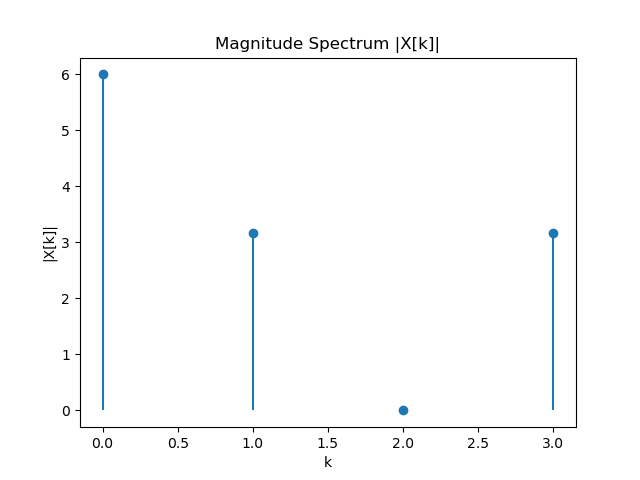
\includegraphics[width=0.7\linewidth]{fig1.png}
\end{center}
\end{frame}


\end{document}
